\section{Spectral and planar preliminaries}\label{sec:preliminaries}

Write $\lambda_D$ for the first Dirichlet eigenvalue of $\Omega$. Both $\mu$ and $\lambda_D$ are positive by the respective Poincar\'e inequalities. Their Rayleigh infima are attained by compactness, and the eigenspaces are finite-dimensional.

The strict separation below is the first-mode case of the Friedlander--Filonov comparison \cite{Friedlander1991,Filonov2005}. We give the plane-wave argument of Filonov in the form needed here, including the strictness that identifies the equality space of the later vector variational principle.

\begin{lemma}\label{lem:gap}
One has $\mu<\lambda_D$.
\end{lemma}
\begin{proof}
Choose a nonzero nonnegative Dirichlet minimizer $\phi$, using absolute values in the Rayleigh quotient. Then $\int_\Omega\phi>0$. Work temporarily over $\C$. For $k\in\R^2$ with $|k|^2=\lambda_D$, put
\[
e_k(x)=e^{ik\cdot x},\qquad
w_k=e_k-\frac{\int_\Omega e_k}{\int_\Omega\phi}\phi.
\]
Each $w_k$ has mean zero. The form $\int(|\grad v|^2-\lambda_D|v|^2)$ vanishes on $e_k$ and $\phi$; its cross term vanishes because $-\Delta e_k=\lambda_De_k$ and $\phi$ has zero trace. Thus every nonzero $w_k$ has Rayleigh quotient $\lambda_D$, proving $\mu\le\lambda_D$.

If equality held, each such $w_k$ would be a Neumann eigenfunction by variational equality. The Euler equation first holds against mean-zero tests and then against all tests, since $w_k$ has mean zero. But distinct plane waves are linearly independent: restrict any finite family to a line segment in an interior ball whose direction gives distinct frequencies. Subtracting multiples of one fixed function leaves their span infinite-dimensional. This contradicts finite eigenspace dimension. The real Neumann inequality and its equality case apply in the complexified space by separating real and imaginary parts.
\end{proof}

We also include the smooth conformal parametrization used throughout the proof; see \cite{Pommerenke1992} for the classical boundary-regularity theory of conformal maps.

\begin{lemma}\label{lem:conformal}
There is a conformal bijection $\Phi:\D\to\Omega$ extending to a smooth diffeomorphism of closures, with $\Phi'\ne0$ on $\overline\D$.
\end{lemma}
\begin{proof}
Identify the plane with $\C$ and fix $a\in\Omega$. Let $l$ solve the harmonic Dirichlet problem with boundary values $\log|z-a|$. It is smooth up to the boundary. Simple connectivity gives a harmonic conjugate $\widetilde l$; its gradient extends smoothly, so the conjugate also extends smoothly in boundary charts. The holomorphic function
\[
m(z)=(z-a)\exp(-l(z)-i\widetilde l(z))
\]
has modulus one on the boundary, modulus less than one inside, and precisely one zero, of order one. Near the boundary, $\log|m|$ is harmonic, negative inside, and zero on the boundary. The boundary point lemma gives a nonzero normal derivative, so $m'$ does not vanish there.

For any $w\in\D$, take a smooth inner approximation of $\Omega$ so close to its boundary that $|m|>|w|$ throughout the omitted collar. Rouch\'e's theorem gives exactly one zero of $m-w$ in that approximation, counting multiplicity, because $m$ has exactly one. There are none in the collar. Thus $m$ is a biholomorphism in the interior. It maps the boundary onto the circle by compactness. Its local boundary inverses imply injectivity there: two boundary preimages would give two nearby interior preimages. The inverse map is the required $\Phi$.
\end{proof}

Throughout, $\Sone=\partial\D$ carries arclength $\dd s$, of total mass $2\pi$.

To bound the dimension of $\V$, we transfer its mean-zero condition to the boundary and use connectedness of the positive and negative sets to control boundary signs.

\begin{lemma}\label{lem:boundary-weight}
There is a fixed smooth positive function $\beta$ on $\Sone$ such that every $v\in\V$ has boundary trace $h_v=v\circ\Phi$ satisfying
\[
\int_{\Sone}\beta h_v\dd s=0.
\]
If $v\ne0$, its boundary trace is nonzero and takes both signs.
\end{lemma}
\begin{proof}
By \Cref{lem:gap}, the Dirichlet problem
\[
(-\Delta-\mu)L=1,\qquad L|_{\partial\Omega}=0
\]
is coercive and has a smooth solution. Testing by its negative part gives $L\ge0$. Hence $-\Delta L=1+\mu L>0$, and the boundary point lemma gives $-\partial_\nu L>0$. Green's identity and the Neumann equation yield
\[
0=\int_\Omega v=-\int_{\partial\Omega}v\,\partial_\nu L
=\int_{\Sone}\beta(s)h_v(s)\dd s,
\quad
\beta=|\Phi'|\,(-\partial_\nu L)\circ\Phi.
\]
If $h_v=0$, then $v\in H^1_0(\Omega)$, and the Dirichlet inequality and $\mu<\lambda_D$ force $v=0$. Positivity of $\beta$ gives the last assertion.
\end{proof}

\begin{lemma}\label{lem:nodal}
For $0\ne v\in\V$, the sets $\{v>0\}$ and $\{v<0\}$ are connected. Its boundary trace cannot have four cyclically ordered points with strictly alternating signs.
\end{lemma}
\begin{proof}
For each component $U$ of a sign set, the function $v_U=v\one_U$ belongs to $H^1(\Omega)$ and has weak gradient $\one_U\grad v$. Indeed it is locally Lipschitz in interior balls: any transition between $U$ and its complement crosses a zero of $v$, so the local Lipschitz bound for $v$ also bounds the zeroed function. This gives the local weak-gradient identity, and the global $L^2$ bounds give global $H^1$ membership. Testing the eigenfunction equation by $v_U$ shows
\[
\int_\Omega|\grad v_U|^2=\mu\int_\Omega|v_U|^2.
\]
If at least three sign components existed, a nonzero linear combination of two restrictions could be chosen mean zero. Disjoint supports show that it attains the quotient $\mu$. It is therefore an eigenfunction, but vanishes on the omitted open component, contradicting interior analyticity. Both sign sets are nonempty, so each is connected.

Four alternating strict signs on the boundary would give a simple arc joining the two positive points, otherwise in the positive interior set, and another joining the negative points in the negative interior set. Such arcs exist by connectedness of open planar sign sets, using short interior end segments and then polygonal paths with loops removed. After applying $\Phi^{-1}$, their endpoints alternate on a circle. Planar separation forces the two arcs to intersect, contrary to their signs; see \Cref{fig:boundary-signs}.
\end{proof}

\begin{figure}[htbp]
  \centering
  \begin{minipage}{.84\textwidth}
  \centering\small
  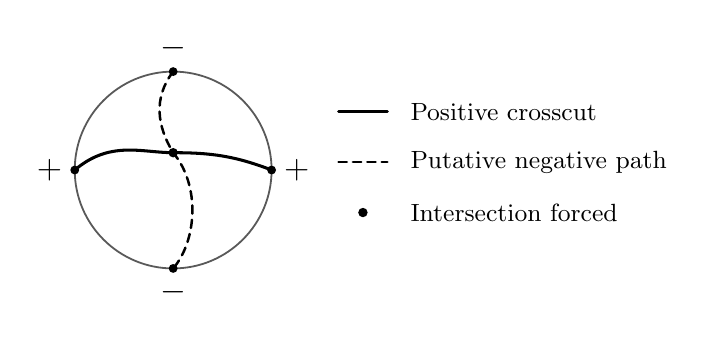
\begin{tikzpicture}[x=1cm,y=1cm,font=\small,
      line cap=round,line join=round]
    \draw[black!65,line width=.65pt] (0,0) circle[radius=1.25];
    \node at (-.67,-.69) {$\D$};

    \draw[line width=1.1pt]
      (-1.25,0) .. controls (-.8,.38) and (-.4,.22) .. (0,.22)
      .. controls (.48,.22) and (.78,.18) .. (1.25,0);

    \draw[line width=.9pt,dash pattern=on 3pt off 2.2pt]
      (0,1.25) .. controls (-.26,.91) and (-.20,.55) .. (0,.22)
      .. controls (.35,-.20) and (.30,-.90) .. (0,-1.25);
    \fill (0,.22) circle[radius=1.7pt];

    \foreach \x/\y in {-1.25/0,1.25/0,0/1.25,0/-1.25}
      \fill (\x,\y) circle[radius=1.6pt];
    \node[font=\large] at (-1.57,0) {$+$};
    \node[font=\large] at (1.57,0) {$+$};
    \node[font=\large] at (0,1.55) {$-$};
    \node[font=\large] at (0,-1.55) {$-$};

    \draw[line width=1.1pt] (2.10,.74) -- (2.72,.74);
    \node[anchor=west] at (2.89,.74) {Positive crosscut};
    \draw[line width=.9pt,dash pattern=on 3pt off 2.2pt]
      (2.10,.10) -- (2.72,.10);
    \node[anchor=west] at (2.89,.10) {Putative negative path};
    \fill (2.41,-.54) circle[radius=1.7pt];
    \node[anchor=west] at (2.89,-.54) {Intersection forced};
  \end{tikzpicture}
  \caption{Connectedness of the positive set gives a crosscut joining the
  $+$ points. It separates the two $-$ points, forcing any negative connecting
  path to meet it. The dashed path illustrates this contradiction; all four
  boundary signs are strict.}
  \label{fig:boundary-signs}
  \end{minipage}
\end{figure}


\Needspace{7\baselineskip}
The following multiplicity bound is due to Nadirashvili \cite[Theorem~3, p.~227]{Nadirashvili1988}; see also \cite[Proposition~2.5]{BanuelosBurdzy1999}. The boundary-sign proof is included for completeness.

\begin{proposition}\label{prop:multiplicity}
The real eigenspace $\V$ has dimension at most two.
\end{proposition}
\begin{proof}
Suppose its dimension is at least three. Since the trace map is injective, choose $0\ne v\in\V$ whose trace $h=h_v$ satisfies
\[
\int_{\Sone}\beta h\cos\theta\dd s
=\int_{\Sone}\beta h\sin\theta\dd s=0,
\qquad s=e^{i\theta}.
\]
It is already orthogonal to $1$ by \Cref{lem:boundary-weight}. Cut the circle at a strictly negative point and write its angles as $(\theta_0,\theta_0+2\pi)$. If $a$ and $b$ are the infimum and supremum of the positive angles, then
\[
\theta_0<a<b<\theta_0+2\pi.
\]
There are no positive values outside $[a,b]$. Nor is there a negative value between $a$ and $b$: positive values on either side of it, together with the cut point, would violate \Cref{lem:nodal}. The function
\[
F(\theta)=\cos\!\left(\theta-\frac{a+b}{2}\right)
-\cos\!\left(\frac{b-a}{2}\right)
\]
is strictly positive on $(a,b)$ and negative outside $[a,b]$ in the cut interval. Consequently $Fh\ge0$ everywhere and $Fh>0$ on a nonempty open set. Thus $\int\beta Fh>0$, contradicting the three orthogonalities.
\end{proof}
